\documentclass[conference]{IEEEtran}
\IEEEoverridecommandlockouts
% The preceding line is only needed to identify funding in the first footnote. If that is unneeded, please comment it out.
%Template version as of 6/27/2024

\usepackage{cite}
\usepackage{amsmath,amssymb,amsfonts}
\usepackage{algorithmic}
\usepackage{graphicx}
\usepackage{textcomp}
\usepackage{xcolor}
\usepackage{tikz}
\usepackage{stfloats} % Optimizes double-column float queues to prevent final page flushing
\usetikzlibrary{shapes.geometric, arrows.meta, positioning, calc}
\def\BibTeX{{\rm B\kern-.05em{\sc i\kern-.025em b}\kern-.08em
    T\kern-.1667em\lower.7ex\hbox{E}\kern-.125emX}}
\begin{document}

\title{Uncertainty-Aware Soft Actor-Critic Control for Quantized Industrial Filling Processes via Kalman Filter Covariance Augmentation\\
}

\author{
    \IEEEauthorblockN{Tania Sarraf}
    \IEEEauthorblockA{\textit{Department of Electrical and Electronics Engineering} \\
    \textit{Marmara University}\\
    Istanbul, Turkiye\\
    taniasarrafjadidian@marun.edu.tr}
    \and
    \IEEEauthorblockN{Ömer Sabri Emeksiz}
    \IEEEauthorblockA{\textit{Department of Computer Engineering} \\
    \textit{Koç University}\\
    Istanbul, Turkiye \\
    oemeksiz24@ku.edu.tr}
    \and
    \IEEEauthorblockN{\vphantom{A}Engin Maşazade}
    \IEEEauthorblockA{\textit{Department of Electrical and Electronics Engineering} \\
    \textit{Marmara University}\\
    Istanbul, Turkiye \\
    engin.masazade@marmara.edu.tr}
    \and
    \IEEEauthorblockN{Suat Selim}
    \IEEEauthorblockA{\textit{BAYKON Industrial Weighing Systems}\\
    Istanbul, Turkiye \\
    sselim@baykon.com}
}

\maketitle

\begin{abstract}
Industrial automated filling processes operating under sensor quantization, high-inertia material landing surges, and unmodeled material density variations present a fundamental challenge to classical control frameworks. While model-free Deep Reinforcement Learning (DRL) can compute nonlinear policies, unguided exploration over raw quantized signals leads to severe gradient instability. Standard stochastic optimization baselines such as Tabular Monte Carlo can identify optimal static switching point but lack online adaptability to dynamic parameter variations. This paper proposes a co-designed uncertainty-aware estimation and control framework (UA-SAC) to address these limitations. A Kalman Filter reconstructs smoothed mass trajectories from $10\,\text{g}$ quantized measurements, providing live state estimates and error covariance diagonals $P_{ii}$ to a downstream Soft Actor-Critic policy. A structured comparative study across four configurations shows that unshielded Vanilla SAC and KF-SAC baselines fail to converge, achieving success rates of $0.20\%$ and $3.70\%$ respectively. A tabular MC baseline achieves $98.70\%$ test success with a MAE of $3.54\,\text{g}$, but its fixed switching threshold fails under extreme density variations. The proposed UA-SAC framework, conditioning its policy on real-time covariance estimates $P_{ii}$, dynamically adjusts its switching point online, thereby achieving $100\%$ success and a MAE of $2.03\,\text{g}$ over $N = 1000$ unseen test episodes within the digital twin environment.
\end{abstract}

\begin{IEEEkeywords}
Industrial filling control, Kalman Filter, Sensor quantization, Soft Actor-Critic, Uncertainty-aware reinforcement learning
\end{IEEEkeywords}

% -------------------------------------------------------
\section{Introduction}
\label{sec:intro}

Automated high-speed mass dispensing and filling systems 
are central to modern manufacturing, chemical processing, 
and packaging industries. The primary objective is to 
maximise throughput while satisfying narrow regulatory 
tolerances. This balance is complicated by nonlinear 
fluid dynamics and a measurement bottleneck: hardware 
scale sensors report data in coarse discrete increments, 
introducing a staircase feedback profile that obscures 
instantaneous mass flow rates.

The industrial benchmark for filling control has 
historically relied on PID controllers \cite{ogata2010}, 
which struggle under multi-stage operation and 
batch-to-batch material parameter drift \cite{sato2010}. 
Early alternatives include iterative learning control 
\cite{an2018,you2018} and tabular reinforcement learning 
\cite{sutton2018}. Notably, \cite{emeksiz2023} introduced 
a data-driven Monte Carlo (MC) benchmark for optimal coarse-to-fine 
switching thresholds, subsequently extended in 
\cite{emeksiz2025} to compare MC against TD-learning and 
Q-learning. While these tabular methods are effective 
under stable, narrow-variation conditions, they rely on 
static thresholds that cannot adapt online to 
batch-to-batch density variations, and they scale poorly 
to higher-dimensional state representations.

The emergence of DRL with deep function approximators 
\cite{mnih2015} offers continuous closed-loop control 
without explicit state discretisation. Among off-policy 
algorithms, SAC \cite{haarnoja2018} is well suited for 
real-world systems by incorporating an entropy term to 
prevent premature policy collapse. However, when exposed 
directly to raw quantized measurements under unmodelled 
parameter drift and landing surges, an unshielded SAC 
agent lacks the predictive estimation layer needed to 
safely navigate asymmetric overshoot constraints, causing 
exploration to stall in a premature-cutoff local minimum.

This motivates retaining classical physics-based state 
estimation alongside DRL. A Kalman Filter (KF) 
\cite{kalman1960}, \cite{simon2006}, \cite{barshalom2001} smooths 
quantized hardware steps via probabilistic relaxation, 
providing continuous kinematic estimates. While several 
prior studies have explored reinforcement learning for 
filter tuning or observer design \cite{tang2021}, \cite{ristic2026}, 
this work investigates the complementary direction in 
which a Kalman filter directly augments a downstream 
SAC controller through state reconstruction and 
uncertainty feedback.

A structured comparative study across four configurations 
validates this architecture. A tabular MC baseline 
\cite{emeksiz2023,sutton2018} establishes the static 
threshold ceiling achievable without online adaptability. 
An intermediate KF-SAC ablation demonstrates that KF 
smoothing alone is insufficient: without real-time 
covariance feedback, the agent remains blind to transient 
filter lag and physical impact shocks. The proposed 
UA-SAC framework addresses this by expanding the SAC 
observation space to include KF state estimates 
$\hat{\mathbf{x}}_k$ alongside the live error covariance 
diagonals $P_{11}, P_{22}, P_{33}$, enabling the policy 
to condition its switching decisions on active estimation 
uncertainty.

The remainder of this paper is organized as follows. 
Section~\ref{sec:env} describes the digital twin. 
Section~\ref{sec:kf} presents the KF design. 
Section~\ref{sec:sac} presents the UA-SAC framework and comparative baselines.
Section~\ref{sec:reward} presents the reward formulation. 
Section~\ref{sec:results} reports experimental results. 
Section~\ref{sec:conclusion} concludes.
% -------------------------------------------------------
\section{Digital Twin Environment}
\label{sec:env}

A digital twin simulates a dual-stage industrial filling loop 
operating under five concurrent physical uncertainty sources. 
The vessel mass evolves at each discrete time step 
$\Delta t = 0.01\,\text{s}$ as:
\begin{equation}
    w_{k+1} = w_k + \left(\dot{m}_u + \alpha \cdot 
    \sigma_\text{proc} \cdot \varepsilon_k\right)\Delta t + \zeta_k,
\end{equation}
where $\varepsilon_k \sim \mathcal{N}(0,1)$, 
$\sigma_\text{proc} = 5.0\,\text{g/s}$, and the valve 
command $u_k \in \{-1,+1\}$ selects between coarse feed 
$\dot{m}_c = 600\,\text{g/s}$ and fine feed 
$\dot{m}_f = 60\,\text{g/s}$.

\textbf{Nonlinear landing surge.} Rapid valve opening at 
episode onset ($k < 15$) produces a time-decaying impact 
transient:
\begin{equation}
    \zeta_k = 20.0 \cdot e^{-k/5.0} \cdot \omega_k, 
    \quad \omega_k \sim \mathcal{U}(0,1).
\end{equation}

\textbf{Stochastic material parameter drift.} A density 
scaling parameter $\alpha \sim \mathcal{U}(0.7,\,1.5)$ is 
sampled once per episode, modelling batch-to-batch 
variations in fluid viscosity and bulk density.

\textbf{Actuation transition delay.} Switching from coarse 
to fine feed ($u_k: +1 \to -1$) induces brief pressure 
transients that locally elevate state estimation error.

\textbf{Residual material-in-flight.} At valve closure, 
airborne material contributes a stochastic terminal mass:
\begin{equation}
    \psi_\text{fall} = \mu_\text{res} + 
    \sigma_{\text{res},k}\,\mathcal{N}(0,1),
\end{equation}
where $\mu_\text{res} = 15.0\,\text{g}$ and the settling 
variance grows with delayed switching:
\begin{equation}
    \sigma_{\text{res},k} = \operatorname{clip}\!\left(
    2.5 + \max\!\left(0,\,
    \tfrac{275 - d_\text{fine}}{275}\right)\cdot 17.5,\;
    2.5,\;20.0\right),
\end{equation}
with $d_\text{fine} = w_\text{final} - w_\text{switch}$ 
denoting the mass accumulated during the fine-feed phase.

\textbf{Hardware measurement quantization.} The sensor 
output is corrupted by additive white noise and rounded to 
the nearest hardware division:
\begin{equation}
    z_k = \left\lfloor\frac{w_k + v_k}{\Delta Q}
    \right\rceil\cdot\Delta Q,
\end{equation}
where $v_k \sim \mathcal{N}(0,\,\sigma_\text{meas}^2)$, 
$\sigma_\text{meas} = 3.0\,\text{g}$, and 
$\Delta Q = 10.0\,\text{g}$.

% -------------------------------------------------------
\section{Robust Adaptive Kalman Filter}
\label{sec:kf}

\subsection{Augmented State-Space Formulation}

The plant state is represented by $\mathbf{x}_k = 
[w_k,\; m_k,\; \alpha_k]^\top \in \mathbb{R}^3$, where 
$w_k$, $m_k$, and $\alpha_k$ denote vessel mass, flow 
rate, and latent density parameter, respectively. The 
discrete-time prediction step is:
\begin{equation}
    \mathbf{x}_{k|k-1} = \mathbf{F}_{k-1}\mathbf{x}_{k-1} 
    + \mathbf{q}_{k-1},
\end{equation}
where $\mathbf{q}_{k-1} \sim \mathcal{N}(\mathbf{0}, 
\mathbf{Q}_k)$ and the state-transition matrix is:
\begin{equation}
    \mathbf{F}_{k-1} = \begin{bmatrix}
        1 & \Delta t & \tfrac{1}{2}u_{k-1}\Delta t^2 \\
        0 & 1        & u_{k-1}\Delta t \\
        0 & 0        & 1
    \end{bmatrix},
    \label{eq:state_transition}
\end{equation}
with $u_{k-1} \in \{+1,-1\}$ denoting the valve command. 
The nominal process noise covariance is 
$\mathbf{Q}_\text{nom} = \operatorname{diag}[1.0,\;50.0,
\;1.0]$ \cite{barshalom2001,simon2006}. To maintain filter 
stability during physical transients, $\mathbf{Q}_k$ is 
scaled by $50\times$ during the landing surge window 
($k < 15$) and by $10\times$ for 10 steps following a 
valve transition. The predicted covariance is:
\begin{equation}
    \mathbf{P}_{k|k-1} = \mathbf{F}_{k-1}
    \mathbf{P}_{k-1|k-1}\mathbf{F}_{k-1}^\top + 
    \mathbf{Q}_k.
\end{equation}

\subsection{Measurement Update under Quantization}

Only vessel mass is measurable, so $\mathbf{H} = 
[1,\,0,\,0]$. The measurement noise variance incorporates 
a quantization error term \cite{simon2006}:
\begin{equation}
    R = \sigma_\text{meas}^2 + \frac{\Delta Q^2}{12} 
    = 3.0^2 + \frac{10.0^2}{12} = 17.33,
\end{equation}
decoupling native sensor noise from discretization error. 
The standard Kalman update equations yield:
\begin{align}
    \tilde{y}_k &= z_k - \mathbf{H}\hat{\mathbf{x}}_{k|k-1}, \\
    S_k         &= \mathbf{H}\mathbf{P}_{k|k-1}
                    \mathbf{H}^\top + R, \\
    K_k         &= \mathbf{P}_{k|k-1}\mathbf{H}^\top 
                    S_k^{-1}, \\
    \hat{\mathbf{x}}_{k|k} &= \hat{\mathbf{x}}_{k|k-1} 
                    + K_k\tilde{y}_k.
\end{align}
The Joseph form is used to guarantee positive 
semi-definiteness \cite{simon2006}:
\begin{equation}
    \mathbf{P}_{k|k} = (\mathbf{I} - K_k\mathbf{H})
    \mathbf{P}_{k|k-1}(\mathbf{I} - K_k\mathbf{H})^\top 
    + K_k R K_k^\top,
\end{equation}
followed by explicit symmetrization 
$\mathbf{P}_{k|k} \leftarrow \tfrac{1}{2}
(\mathbf{P}_{k|k} + \mathbf{P}_{k|k}^\top)$. The 
diagonal entries $P_{11,k},\,P_{22,k},\,P_{33,k}$ are 
extracted and passed to the downstream SAC policy as 
live uncertainty features.

% -------------------------------------------------------
\section{Uncertainty-Aware Control Framework and Baselines}
\label{sec:sac}
% -------------------------------------------------------

\subsection{Maximum Entropy Objective}

Standard RL maximises the discounted cumulative reward $\sum_t \gamma^t r(s_t, a_t)$. SAC augments this with an entropy bonus \cite{haarnoja2018}:
\begin{equation}
    J(\pi) = \sum_{t=0}^{T} \mathbb{E}_{(s_t, a_t)\sim\rho_\pi}\!\left[r(s_t, a_t) + \alpha_\text{SAC}\mathcal{H}(\pi(\cdot|s_t))\right],
\end{equation}
where $\mathcal{H}(\pi(\cdot|s_t)) = -\int \pi(a|s)\log\pi(a|s)\,da$ and $\alpha_\text{SAC}$ is a learnable temperature coefficient. Maximising this objective provides robust exploration, implicit gradient regularisation, and multi-modal adaptability, critical properties in the presence of quantization noise and fluid landing surges \cite{haarnoja2018}.

\subsection{Twin-Critic Architecture}

To mitigate Q-value overestimation, two independent soft Q-networks $Q_{\phi_1},\, Q_{\phi_2}$ are trained concurrently by minimising the mean squared Bellman error. The target value integrates next-state entropy:
\begin{equation}
\begin{split}
    \hat{Q}(s_k, a_k) = \, & r_k + \gamma \mathbb{E}_{s_{k+1}} \! \left[ \min_{j} Q_{\bar{\phi}_j}(s_{k+1}, a_{k+1}) \right. \\
    & \left. - \,\alpha_{\text{SAC}} \log \pi_\theta(a_{k+1} | s_{k+1}) \right].
\end{split}
\end{equation}
Target networks are updated via exponential moving average with $\tau_\text{soft} = 0.005$.

\subsection{Observation Space and Action Interface}

The actor processes a 7-dimensional uncertainty-aware state vector:
\begin{equation}
    \mathbf{s}_k = \left[\hat{w}_k,\; \hat{m}_k,\; \hat{\alpha}_k,\; P_{11,k},\; P_{22,k},\; P_{33,k},\; w_{\text{target}} - \hat{w}_k\right]^\top,
\end{equation}
where $\hat{w}_k, \hat{m}_k, \hat{\alpha}_k$ are KF estimated states, $P_{ii,k}$ are live covariance diagonals providing real-time filter uncertainty to the policy, and the final term is the explicit goal distance. The reparameterisation trick maps actor output to a continuous action $a_k = \tanh(\mu_\theta(s_k) + \sigma_\theta(s_k)\odot\epsilon_k)$, $\epsilon_k \sim \mathcal{N}(0, \mathbf{I})$, enforcing $a_k \in [-1.0, 1.0]$. This maps to the binary valve command:
\begin{equation}
    u_k = \begin{cases} +1.0 & \text{if } a_k \geq 0 \quad (\text{coarse feed}) \\ -1.0 & \text{if } a_k < 0 \quad (\text{fine feed}) \end{cases}.
\end{equation}
The twin critic networks operate on an 8-dimensional space $\mathbb{R}^7 \times \mathbb{R}^1$. The target entropy is fixed at $\mathcal{H}_\text{target} = -2.5$ to maintain aggressive exploration scaling throughout training.

\begin{figure}[!t]
\centering
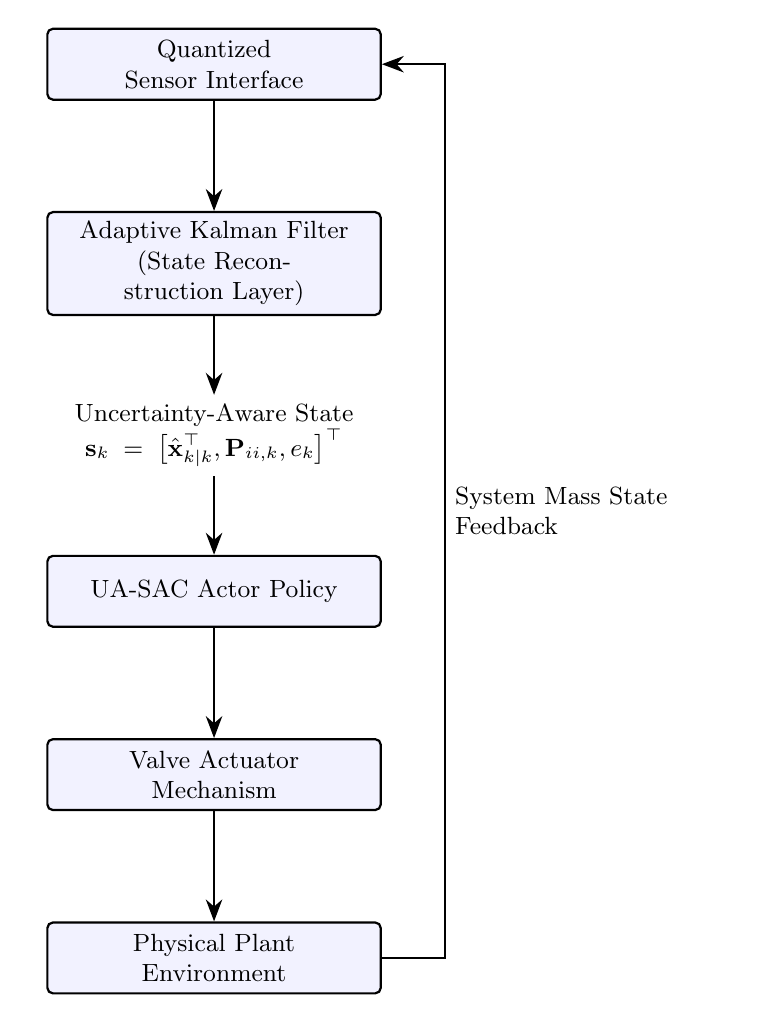
\begin{tikzpicture}[
    node distance=1.4cm,
    auto,
    block/.style={
        rectangle, 
        draw, 
        thick, 
        fill=blue!5, 
        text width=4.0cm, 
        align=center, 
        minimum height=0.9cm,
        rounded corners=2pt,
        font=\small
    },
    signal/.style={
        rectangle, 
        draw=none, 
        fill=none, 
        text width=4.5cm, 
        align=center, 
        minimum height=0.6cm,
        font=\small
    },
    arrow/.style={-{Stealth[scale=1.2]}, thick}
]

    % Place Nodes sequentially with distinct padding tracking
    \node [block] (sensor) {Quantized\\Sensor Interface};
    
    \node [block, below=of sensor] (kf) {Adaptive Kalman Filter\\(State Reconstruction Layer)};
    
    % increased spacing specifically for this label area to avoid overlaps
    \node [signal, below=1.0cm of kf] (state) {Uncertainty-Aware State\\$\mathbf{s}_k = \left[\hat{\mathbf{x}}_{k|k}^\top, \mathbf{P}_{ii,k}, e_k\right]^\top$};
    
    \node [block, below=1.0cm of state] (actor) {UA-SAC Actor Policy};
    
    \node [block, below=of actor] (valve) {Valve Actuator\\Mechanism};
    
    \node [block, below=of valve] (plant) {Physical Plant\\Environment};

    % Draw Directed Connections
    \draw [arrow] (sensor) -- (kf);
    \draw [arrow] (kf) -- (state);
    \draw [arrow] (state) -- (actor);
    \draw [arrow] (actor) -- (valve);
    \draw [arrow] (valve) -- (plant);

    % Right Side Loopback Feedback Layout
    \draw [arrow] (plant.east) -- ++(0.8,0) |- (sensor.east)
        node[pos=0.25, right, font=\small, text width=3.5cm] {System Mass State Feedback};

\end{tikzpicture}
\caption{System block diagram illustrating the Uncertainty-Aware architecture where raw quantized observations are mapped into a smooth, uncertainty-aware feature vector to guide actor policy decisions.}
\label{fig:architecture_flow}
\end{figure}

\subsection{Comparative Ablation State Structures}
To mathematically evaluate the individual contributions of continuous filtering and active uncertainty features, the state inputs are altered into two distinct ablation spaces:
\begin{itemize}
    \item \textbf{Vanilla SAC Baseline ($\mathbf{s}_{k,\text{van}} \in \mathbb{R}^3$):} A model-free vector mapping raw, discrete feedback steps directly into actions, blind to kinematics and tracking variances:
    \begin{equation}
        \mathbf{s}_{k,\text{van}} = \left[z_k,\; \Delta z_k,\; w_{\text{target}} - z_k\right]^\top,
    \end{equation}
    where $z_k$ is the raw quantized measurement from the physical hardware scale and $\Delta z_k = z_k - z_{k-1}$.
    \item \textbf{KF-SAC Baseline ($\mathbf{s}_{k,\text{kf}} \in \mathbb{R}^4$):} An intermediate, uncertainty-blind vector shielded by smoothed continuous tracking states but devoid of error covariance data:
    \begin{equation}
        \mathbf{s}_{k,\text{kf}} = \left[\hat{w}_k,\; \hat{m}_k,\; \hat{\alpha}_k,\; w_{\text{target}} - \hat{w}_k\right]^\top.
    \end{equation}
\end{itemize}
The twin critic networks adapt structural dimensions to match, operating on input layers of $\mathbb{R}^3 \times \mathbb{R}^1$ for Vanilla SAC and $\mathbb{R}^4 \times \mathbb{R}^1$ for KF-SAC.

\subsection{Tabular Monte Carlo Threshold Baseline}
\label{sec:mc}

To complement these DRL-specific state ablations with a non-neural stochastic optimization benchmark, a tabular first-visit Monte Carlo agent is implemented on the digital twin environment described in Section~\ref{sec:env}. Rather than per-step binary valve commands, the agent operates on a \emph{macro-action} formulation: at the start of each episode, a single coarse-to-fine switching threshold $w_\text{sw} \in \{350, 360, \ldots, 650\}\,\text{g} $ is selected from a discrete action set with a $10\,\text{g}$ resolution. The environment then executes the full filling trajectory deterministically under the chosen threshold rule, wherein it applies a coarse feed ($u_k = +1.0$) whenever the raw measurement $z_k < w_\text{sw}$, and snapping to a fine feed ($u_k = -1.0$) the instant $z_k \ge w_\text{sw}$, ultimately returns the episodic cumulative reward as a scalar signal.

The state is represented by the quantized vessel mass $z_k$ rounded to the nearest $10\,\text{g}$ step, consistent with the hardware scale resolution in \cite{emeksiz2023}. Since the optimal macro threshold selection is independent of the instantaneous weight mid-episode, a unified entry-point state key $s_0 = (0)$ is used. This reduction simplifies the sequential optimization task into a single-state, multi-armed bandit problem over the discrete threshold action domain.

State-action values are updated via incremental first-visit Monte Carlo averaging \cite{sutton2018}:
\begin{equation}
    Q(s_0, a) \leftarrow Q(s_0, a) + \frac{1}{n(a)} \bigl(G - Q(s_0, a)\bigr),
\end{equation}
where $G$ is the episodic return and $n(a)$ is the cumulative visit count for threshold action $a$. Action selection follows an $\epsilon$-greedy policy with $\epsilon_0=1.0$, $\epsilon_\text{min}=0.05$, and a decay rate of $0.998$ per episode, matching the hyperparameter configuration in \cite{emeksiz2023, emeksiz2025}. The baseline agent is trained for 3000 episodes on the identical digital twin environment used across all SAC configurations, with the tracking rewards governed by the formulations outlined in Section~\ref{sec:reward}.

% -------------------------------------------------------
\section{Reward Formulation}
\label{sec:reward}

\subsection{Per-Step Rewards}

The Vanilla SAC baseline receives a per-step reward 
blind to estimation uncertainty:
\begin{equation}
    r_{k,\text{van}} = \rho_\text{time} + 
    \psi_\text{chatter} + \psi_\text{early}.
\end{equation}
The KF-SAC and UA-SAC agents additionally penalize 
KF tracking error at each step:
\begin{equation}
    r_{k,\text{kf}} = r_{k,\text{UA}} = \rho_\text{time} 
    - \lambda \cdot \min(|\hat{w}_k - w_k|,\;100.0) 
    + \psi_\text{chatter} + \psi_\text{early},
\end{equation}
where $\lambda = 0.02$. The MC baseline does not 
use per-step rewards; instead, the full episodic 
cumulative reward is returned as a single scalar 
at episode termination, consistent with the 
macro-action formulation in Section~\ref{sec:mc}.

\subsection{Asymmetric Operational Time Cost}

To balance throughput against overshoot risk, 
$\rho_\text{time}$ is a state-dependent cost:
\begin{equation}
    \rho_\text{time} = \begin{cases}
        -0.01 & \text{coarse feed, } \hat{w}_k \leq 
                450\,\text{g} \\
        -5.00 & \text{coarse feed, } \hat{w}_k > 
                450\,\text{g} \\
        -1.50 & \text{fine feed}
    \end{cases}.
\end{equation}
The elevated penalty above $450\,\text{g}$ discourages 
prolonged coarse-feed operation near the target.

\subsection{Actuation Transition Regularization}

A chatter penalty prevents fine-to-coarse reversals:
\begin{equation}
    \psi_\text{chatter} = \begin{cases} 
        -50.0 & \text{if } u_{k-1}=-1 \text{ and } 
                u_k=+1 \\ 
        0.0   & \text{otherwise} 
    \end{cases}.
\end{equation}
A quadratic penalty discourages premature switching:
\begin{equation}
    \psi_\text{early} = \begin{cases} 
        -0.008(400 - \hat{w}_k)^2 & \text{switch at } 
        \hat{w}_k < 400\,\text{g} \\ 
        0.0 & \text{otherwise} 
    \end{cases}.
\end{equation}

\subsection{Terminal Reward}

\begin{figure}[!t]
    \centering
    \vspace{-0.1cm}
    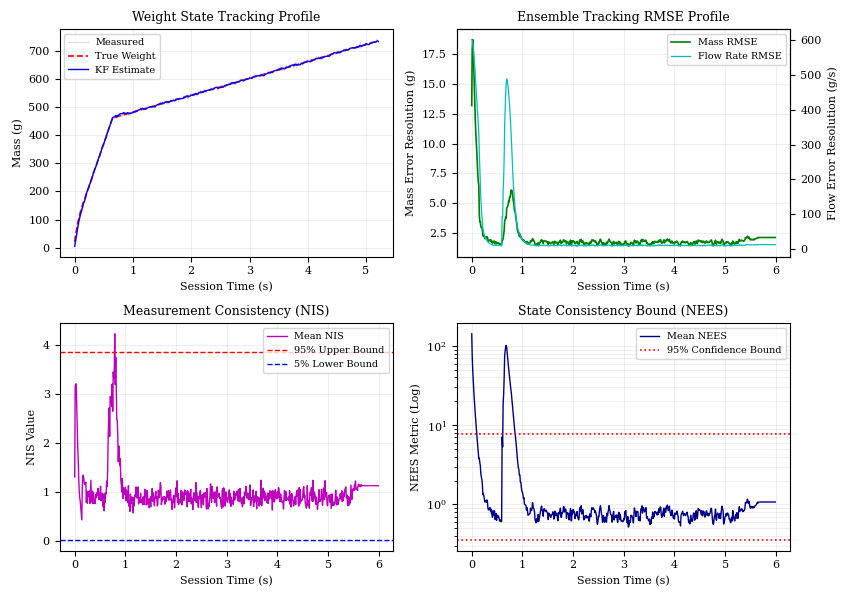
\includegraphics[width=1.0\columnwidth]{filter_test.png}
    \vspace{-0.2cm}
    \caption{Kalman Filter Monte Carlo validation (100 trials): \textbf{(a)} weight state tracking, \textbf{(b)} ensemble RMSE, \textbf{(c)} NIS consistency, and \textbf{(d)} NEES confidence tunnel.}
    \label{fig:kf_mc}
    \vspace{-0.15cm}
\end{figure}

All four agents share the same terminal reward 
structure applied at episode completion:
\begin{equation}
    R_\text{term} = \begin{cases}
        600 + \max(0,\,(800-k_f)\cdot 0.5) & 
        740 \leq w_f \leq 760\,\text{g} \\[2pt]
        -100\ln(1 + 5(w_f - 760)) - 800 & 
        w_f > 760\,\text{g} \\[2pt]
        -500 & w_f < 740\,\text{g}
    \end{cases}
\end{equation}
where $k_f$ is the terminal step count and $w_f$ 
is the final vessel mass. The success bonus 
incentivizes fast filling cycles, while the 
logarithmic overflow penalty provides a smooth 
gradient discouraging overfill. The underflow 
penalty enforces the lower tolerance boundary. 
The TTT reference:
\begin{equation}
    \text{TTT}_k = \frac{w_\text{target} - 
    \hat{w}_k}{\hat{m}_k}
\end{equation}
is computed at each step by the KF-equipped agents 
to inform internal scheduling but does not appear 
directly in the reward signal.

% -------------------------------------------------------
\section{Experimental Results}
% -------------------------------------------------------
\label{sec:results}

\subsection{KF Monte Carlo Validation}

Prior to control training, the KF was validated over
100 Monte Carlo trials on a representative dosing
session ($0$--$6\,\text{s}$). As shown in
Fig.~\ref{fig:kf_mc}, the KF estimate closely tracks
the true vessel mass despite quantization
\cite{simon2006}. The ensemble RMSE for mass and flow
rate converges to near-zero after the initial transient
($t < 1\,\text{s}$), the mean NIS remains within the
95\% chi-squared bounds throughout, and the mean NEES
settles within the 95\% confidence interval after
initial surge transients, confirming filter consistency
under sensor quantization \cite{simon2006}.

\subsection{Training Configuration}

All SAC-based agents used identical hyperparameters:
two hidden layers of 256 neurons, learning rate
$3 \times 10^{-4}$, batch size 256, replay buffer
capacity $100\,000$, and discount factor $\gamma=0.99$.
All four frameworks were trained for 3000 episodes
using the same random seed and digital twin. Vanilla
SAC operated on raw quantized observations; KF-SAC and
UA-SAC used KF state estimates. The MC agent used
first-visit Monte Carlo with $\epsilon$-greedy
exploration ($\epsilon_0=1.0$, $\epsilon_\text{min}=
0.05$, decay $0.998$/episode).

\subsection{Quantitative and Learning Dynamics Analysis}

\begin{table*}[!t]
\renewcommand{\arraystretch}{1.3}
\caption{Control and Estimation Metrics Comparison}
\label{tab:comparison}
\centering
\begin{tabular}{lcccc}
\hline\hline
\bfseries Metric & \bfseries Vanilla SAC & \bfseries KF-SAC & \bfseries Tabular MC & \bfseries UA-SAC \\
\hline
Total episodes          & 3000    & 3000    & 3000    & 3000 \\
Success rate            & 0.20\%  & 3.70\%  & 92.53\% & \textbf{99.47\%} \\
Overflow rate           & 0.00\%  & 3.53\%  & 2.43\%  & 0.10\% \\
Underflow rate          & 99.80\% & 92.77\% & 5.03\%  & 0.43\% \\
MAE (g)                 & 284.68  & 299.98  & 4.90    & \textbf{3.07} \\
Final weight std (g)    & 19.12   & 101.12  & 8.60    & \textbf{18.15} \\
Switch point median (g) & 110.00  & 5.14    & 490.00  & 447.30 \\
Mean KF NIS             & N/A     & 0.09    & N/A     & 0.99 \\
Mean KF NEES            & N/A     & 0.57    & N/A     & 3.58 \\
\hline\hline
\end{tabular}
\end{table*}

\begin{figure*}[!t]
    \centering
    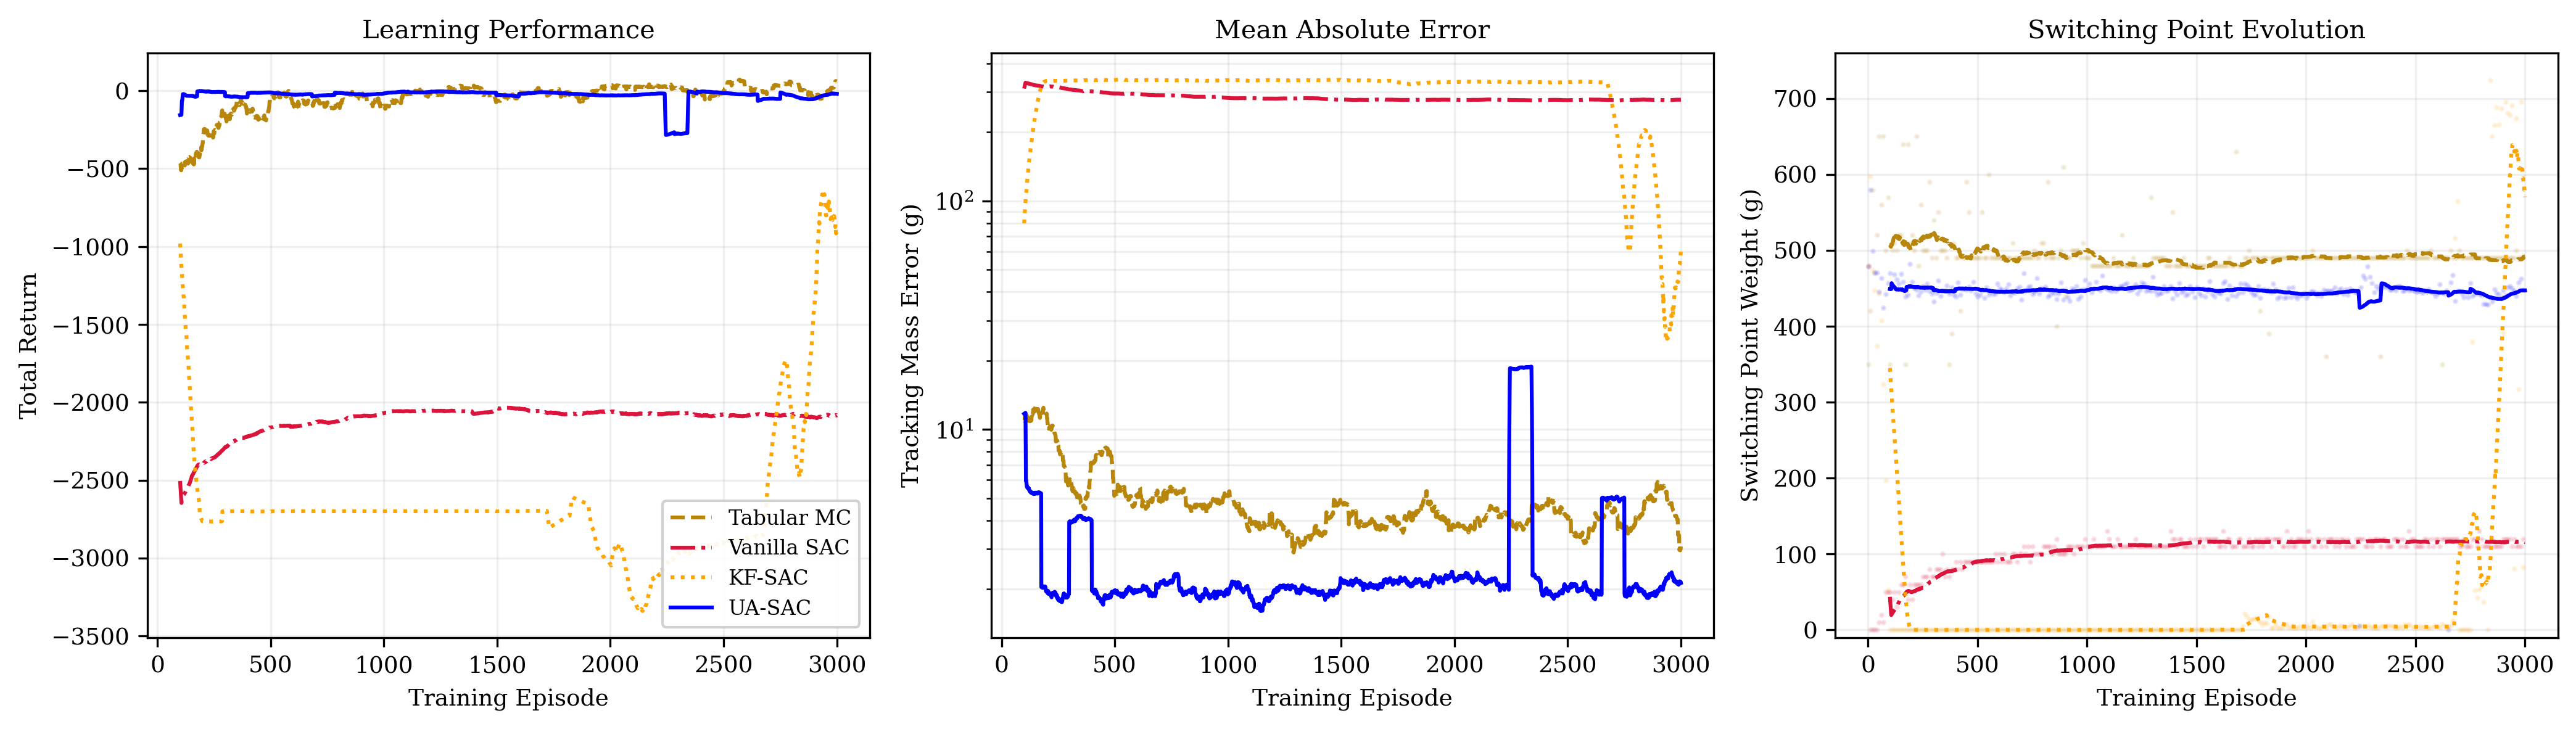
\includegraphics[width=2.0\columnwidth]{unified_training_comparison.png}
    \caption{Training curves across a 3000-episode horizon for Vanilla SAC, KF-SAC, Tabular MC, and UA-SAC.}
    \label{fig:grid_comparison}
\end{figure*} % FIXED: Closing tag repaired from rogue \end{figure*> bracket

Table~\ref{tab:comparison} and
Fig.~\ref{fig:grid_comparison} summarise the
comparative results. Vanilla SAC, operating on raw
quantized inputs, experiences critic loss saturation
within the first episodes and stalls at a median switch
point of $110.00\,\text{g}$, yielding a $99.80\%$
underflow rate throughout training. Adding KF state
estimates via KF-SAC does not resolve convergence: the policy switches prematurely at a median of 5.14 g, triggering the filter noise inflation schedule and driving the estimator into an over-conservative regime, as the absence of covariance feedback prevents the agent from distinguishing between reliable state estimates and transient estimation uncertainty. This suppresses mean NIS to
$0.09$ and NEES to $0.57$, well below theoretical
expectations, and the MAE profile stalls for all 3000
episodes. The MC baseline avoids per-step optimisation
by selecting a fixed threshold per episode, converging
to a median of $490.00\,\text{g}$ with a $92.53\%$
success rate and MAE of $4.90\,\text{g}$. However, its
static threshold cannot adapt within an episode,
resulting in a $2.43\%$ overflow and $5.03\%$
underflow rate under batch-to-batch density drift.
UA-SAC achieves stable convergence to a median switch
point of $447.30\,\text{g}$, yielding a final training 
success rate of $99.47\%$ and an MAE of $3.07\,\text{g}$, 
with filter diagnostics confirming consistent estimation 
(mean NIS $=0.99$, NEES $=3.58$).

\subsection{Test Phase Evaluation (Frozen Policy)}
\label{sec:test}

Given that Vanilla SAC and KF-SAC failed to achieve
viable training convergence, frozen-policy evaluation
is conducted for UA-SAC and the MC baseline only.
UA-SAC achieves a $100\%$ success rate with a MAE of
$2.03\,\text{g}$ relative to ground-truth vessel mass
within the digital twin environment. The error is below the 10 g sensor quantization step within the digital twin environment, demonstrating that the KF can reconstruct latent continuous states more accurately than the raw measurements themselves and achieve sub-resolution estimation accuracy. The MC baseline achieves $98.70\%$ success with
a MAE of $3.54\,\text{g}$. Its switch-point standard
deviation of $\sigma_\text{sw}=0.00\,\text{g}$ confirms
a fixed cutoff regardless of batch conditions, which
accounts for the $1.30\%$ failure rate under extreme
density drift. UA-SAC's $\sigma_\text{sw}=5.92\,
\text{g}$ under deterministic inference reflects
state-dependent adaptation: the live $P_{ii,k}$
covariance terms shift the cutoff threshold in response
to varying material density $\alphapref_k$, confirming that
the uncertainty features carry actionable information
the frozen policy correctly exploits.

\begin{table}[!t]
\renewcommand{\arraystretch}{1.3}
\caption{Frozen Policy Test Results ($N=1000$ Episodes)}
\label{tab:test}
\centering
\begin{tabular}{lcc}
\hline\hline
\bfseries Metric & \bfseries Tabular MC &
\bfseries UA-SAC \\
\hline
Test episodes ($N$) & 1000 & 1000 \\
Success rate & 98.70\% & \textbf{100.00\%} \\
MAE (g) & 3.54 & \textbf{2.03} \\
Mean switch point $\mu_\text{sw}$ (g) & 490.57 & 447.30 \\
Switch point std $\sigma_\text{sw}$ (g) & 0.00 & \textbf{5.92} \\
\hline\hline
\end{tabular}
\end{table}

% -------------------------------------------------------
\section{Conclusion and Future Work}
\label{sec:conclusion}

This paper presented UA-SAC, a co-designed estimation 
and control framework that injects real-time KF error 
covariance diagonals $P_{ii}$ directly into a 
maximum-entropy SAC policy. A structured comparative 
study showed that vanilla and uncertainty-blind KF-SAC 
baselines fail to converge under sensor quantization 
and parameter drift, while a tabular MC baseline 
achieves competitive performance through a static 
switching threshold but cannot adapt to batch-to-batch 
density variations. Frozen-policy evaluations over unseen test episodes confirmed that 
UA-SAC eliminates boundary-tolerance violations and minimizes mass tracking 
error down to sub-quantization levels within the digital twin environment. 
This performance establishes that the policy converges on an adaptive, 
state-dependent switching behavior driven entirely by live covariance 
feedback rather than a rigid, hard-coded threshold rule.

Future work will investigate a communication-aware extension in which Kalman filter covariance governs event-triggered state transmissions, allowing uncertainty to inform both control and communication decisions.
\section*{Acknowledgments}

The authors acknowledge the use of Gemini (Google AI) to assist in generating the Python scripts used for the experimental evaluation in Section \ref{sec:sac} and Section \ref{sec:results}. Additionally, during the preparation of this manuscript, the tool was utilized for editing and grammatical enhancement to improve overall text readability. The authors have rigorously tested and verified all generated code, reviewed all structural and textual modifications, and assume full responsibility for the final content of the publication.
% -------------------------------------------------------
% -------------------------------------------------------
\bibliographystyle{IEEEtran}
\bibliography{references}
% -------------------------------------------------------


\end{document}